\documentclass{report}
\usepackage{graphicx} % Required for inserting images
\usepackage[margin=1in, includefoot]{geometry}
\usepackage[hidelinks]{hyperref}
\usepackage{color}
\usepackage{array}
\usepackage{caption}

\setlength{\tabcolsep}{18pt}
\renewcommand{\arraystretch}{1.5}
\setlength{\arrayrulewidth}{0.5mm}



\begin{document}

\begin{titlepage}
    
    \begin{center}
        \begin{figure}
            \centering
            \vspace{0.75in}
            
\includegraphics[width=0.75\linewidth]{logo.png}
            \vspace{1in}
        \end{figure}

        \textsc{ \Large { Computer Science Lab (B201C) Report}}\\
        [0.75in]
        \line(1,0){450}\\
        [3mm]
        \huge{\bf A Descriptive Report On: \\
        Portfolio Design, CV and Python Project}
        \line(1,0){450}\\
        [2cm]

        \large {Tushar Bhardwaj\\ (GH1040649)}
        
    \end{center}
\end{titlepage} 

% Following line is for ToC
\tableofcontents
\newpage

% Chapter 1 : Introduction

\chapter{Introduction}
A  student portfolio is indeed a necessary aspect in current times which is not only limited to job hunt but also provides a chance for self-assessment, giving the student insight into their progress in general, which may help in their personal growth. \\
\par
This report revolves around the criteria, aspects, features, and procedures of how I made my portfolio website, Curriculum Vitae in LaTeX, and why I chose the design I chose.\\
Furthermore, the report dives deeper, exploring the tools used in the process and then will come to an end showcasing what I learnt and how it will help me in my professional development. \par
This report also encloses all the links to different parts of the project i.e., the links to :
\begin{enumerate}
   
    \item Portfolio website
    \item GitHub Repository of the Portfolio website
    \item Curriculum Vitae PDF
    \item GitHub Repository of .tex file of CV
    \item GitHub Repository of .tex file of this Report
    \item GitHub Repository of Python Project {\bf Automated-Plagiarism-Checker}
    \item Demo video of Python Project
    
\end{enumerate}

% Declaration of Objective
\section{Objective}
The only objective of this report file is to provide a combined summary of all the different aspects like portfolio website, professional CV, and gaining hands-on experience in LaTeX. By doing so, students like me will make a professional presentation online as a student applying for a working-student position in a company.


\newpage
\chapter{Projects \& Links}


\section{Portfolio Website} \par
{\bf Link : \href{https://tusharbhardwaj.com}{\color{blue}tusharbhardwaj.com}}\\
{\bf GitHub: \href{https://github.com/tusharrbhardwaj/myportfolio}{\color{blue}Source Code}} \\ \par
This is my portfolio website, which I myself made from scratch using HTML5 and raw CSS3 along with a minimal use of Javascript. The portfolio website is hosted on my personal domain, which adds to the authenticity of my appearance. It is hosted on \href{https://app.netlify.com}{\color{blue}netlify}, which is a reliable hosting platform. This website is fully responsive and can behave as the demanded media-size of the screen.
These are some snapshots of my portfolio for a better understanding of the design.
 
\begin{figure}[h]
    \centering
    \begin{minipage}{0.49\textwidth}
        \centering
        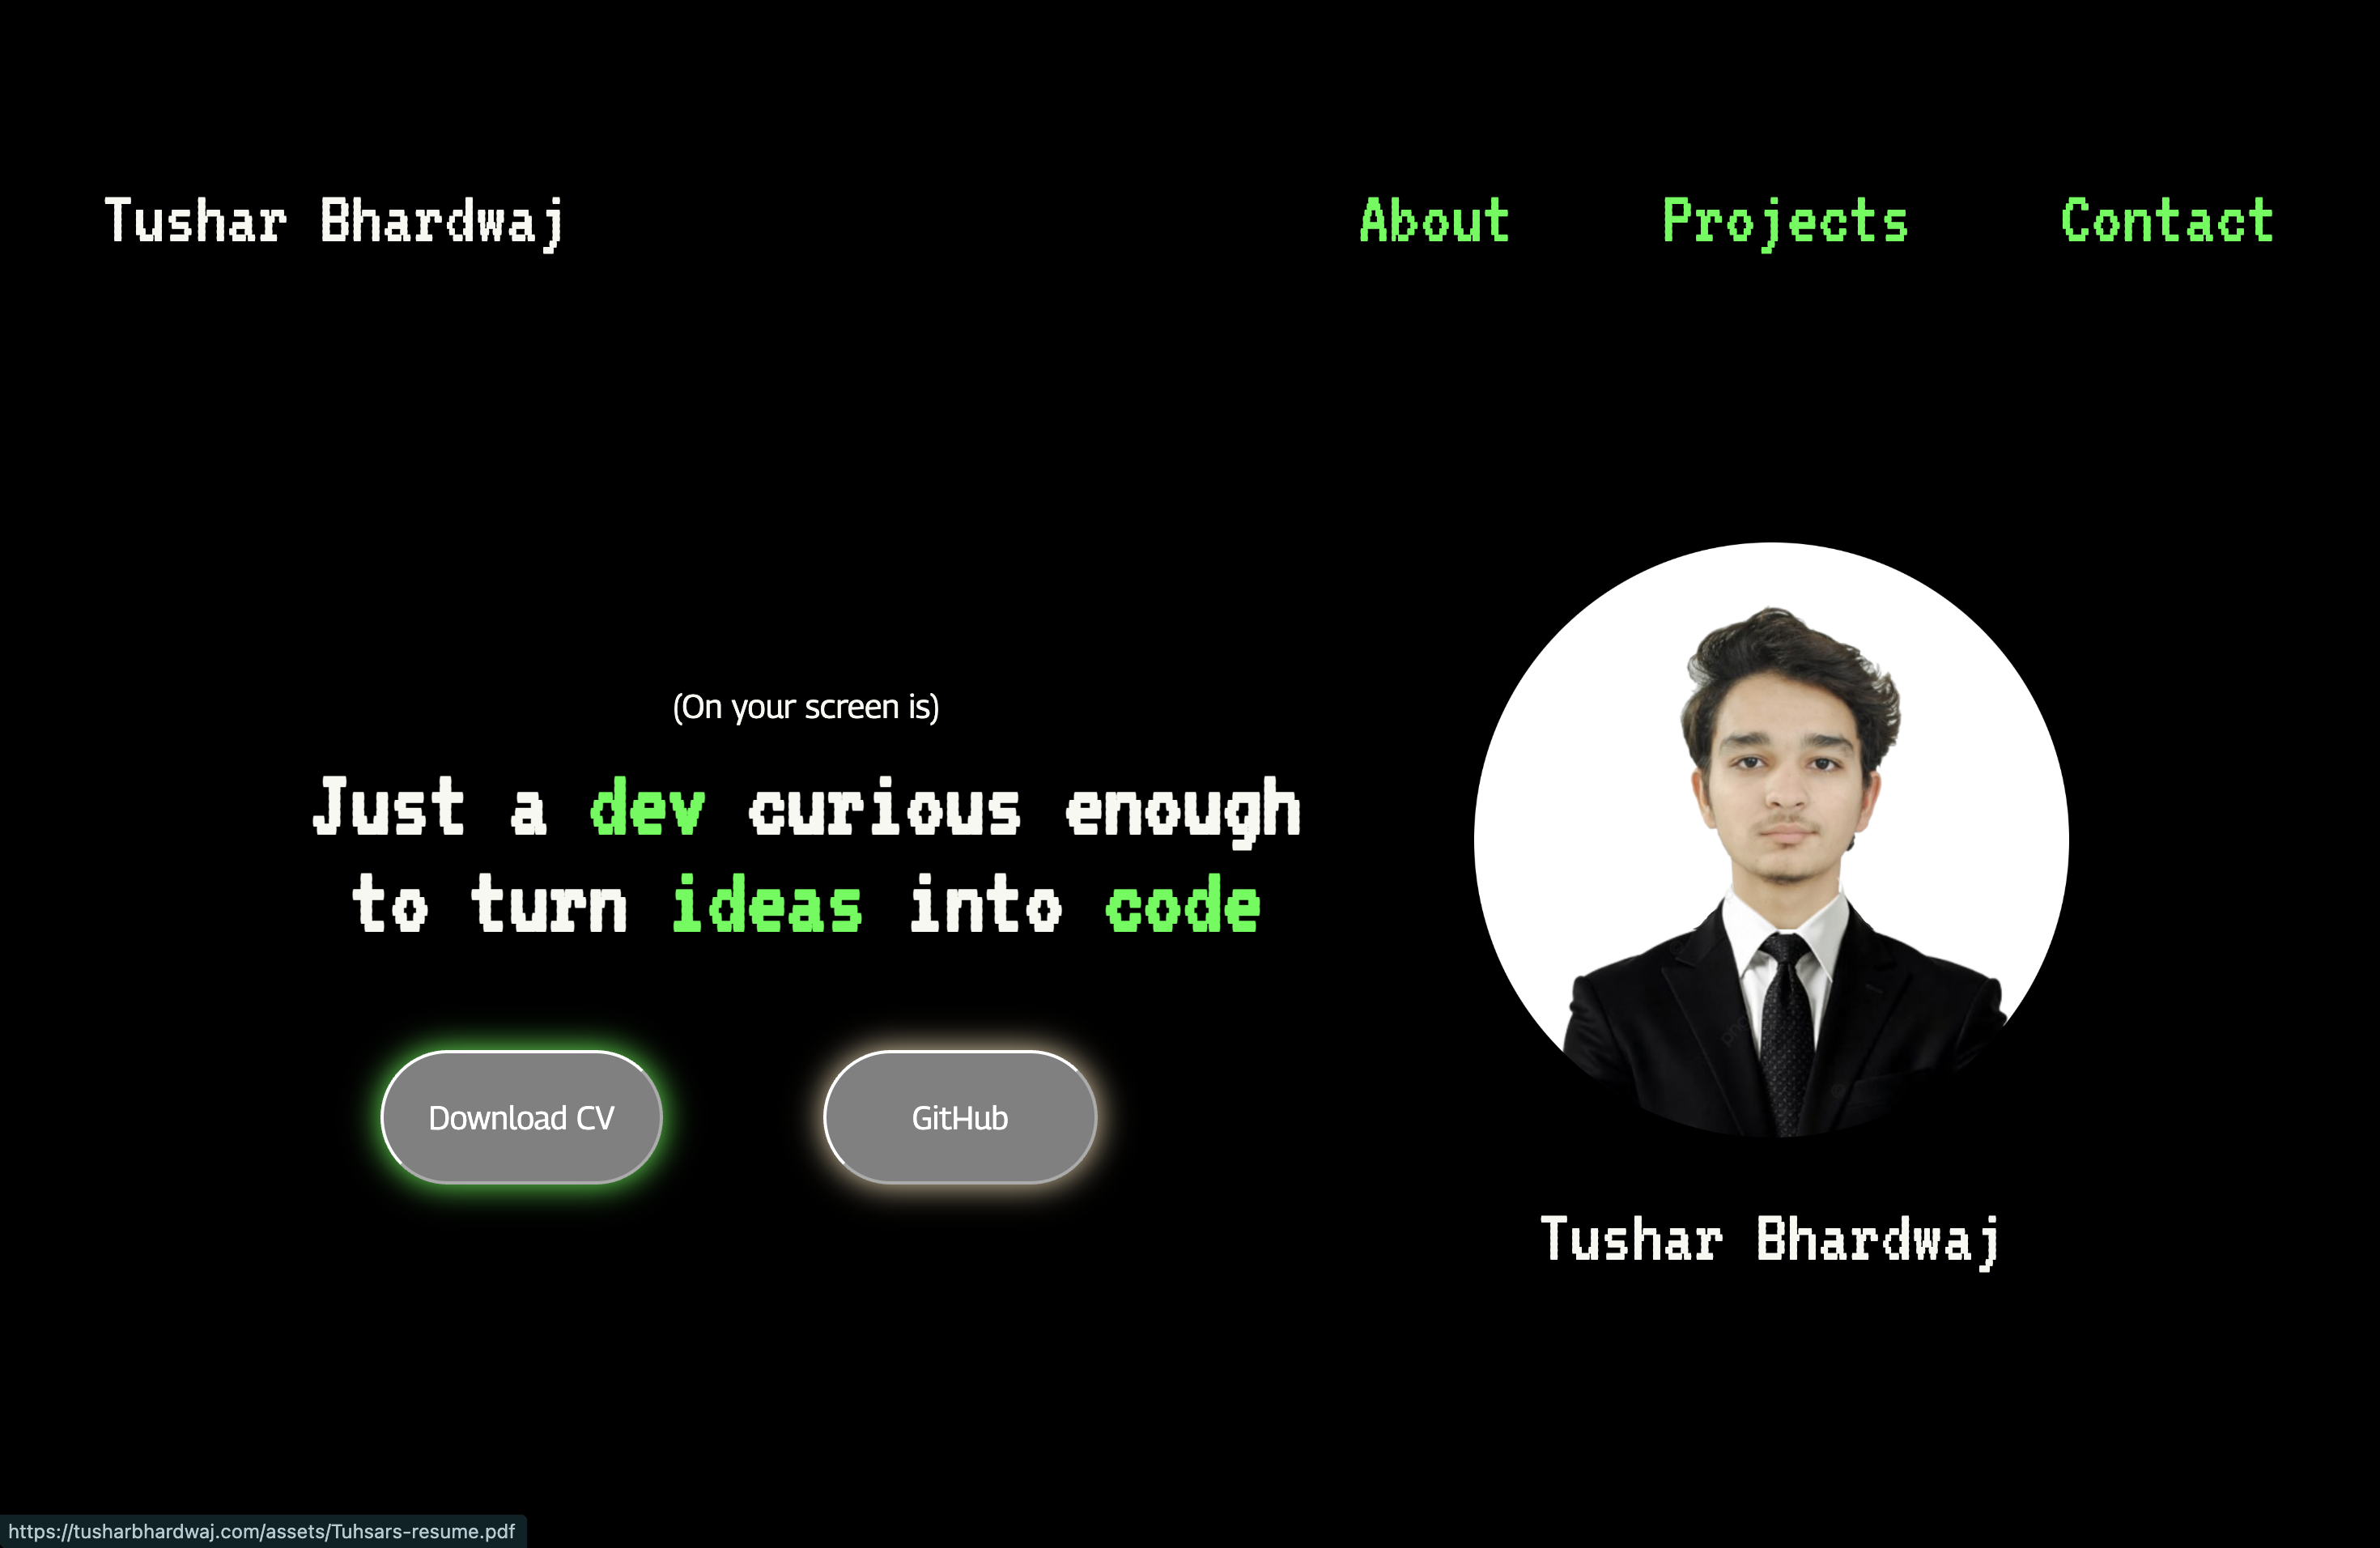
\includegraphics[width=1\linewidth]{webshots/front.png}
    \end{minipage}
    \begin{minipage}{0.49\textwidth}
        \centering
        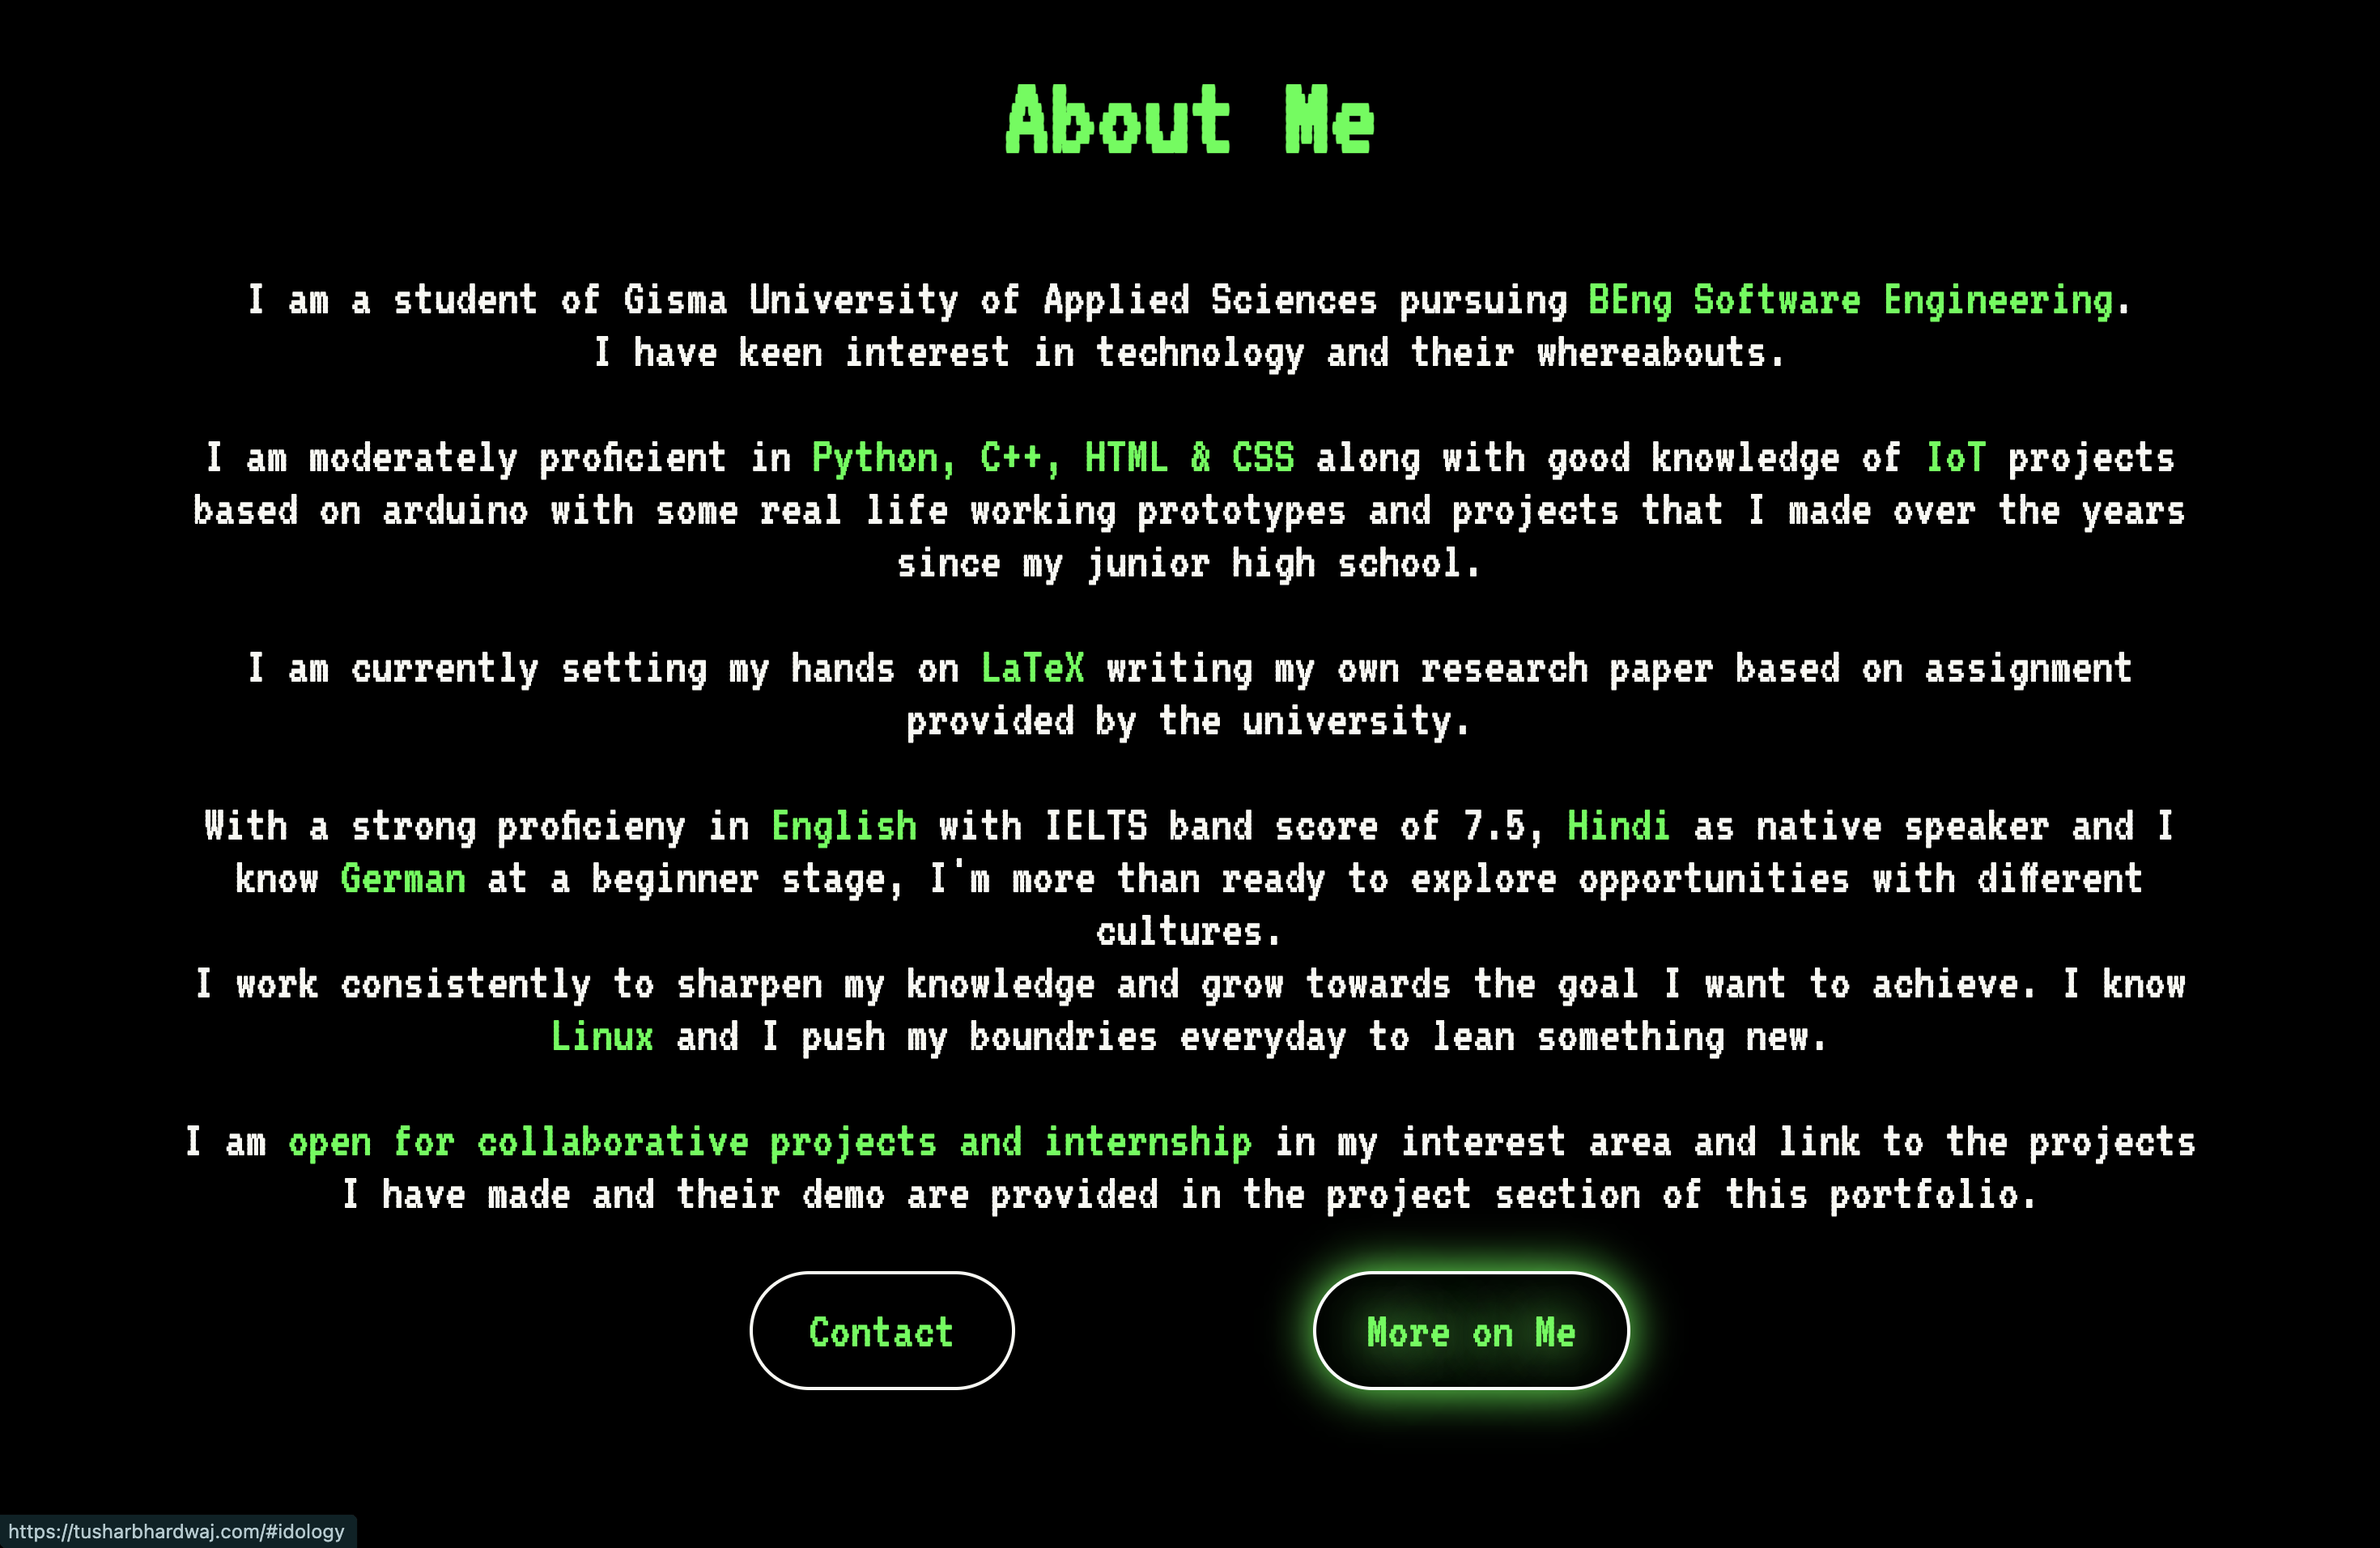
\includegraphics[width=1\linewidth]{webshots/about.png}  
    \end{minipage}
    \\
    \begin{minipage}{0.49\textwidth}
        \centering
        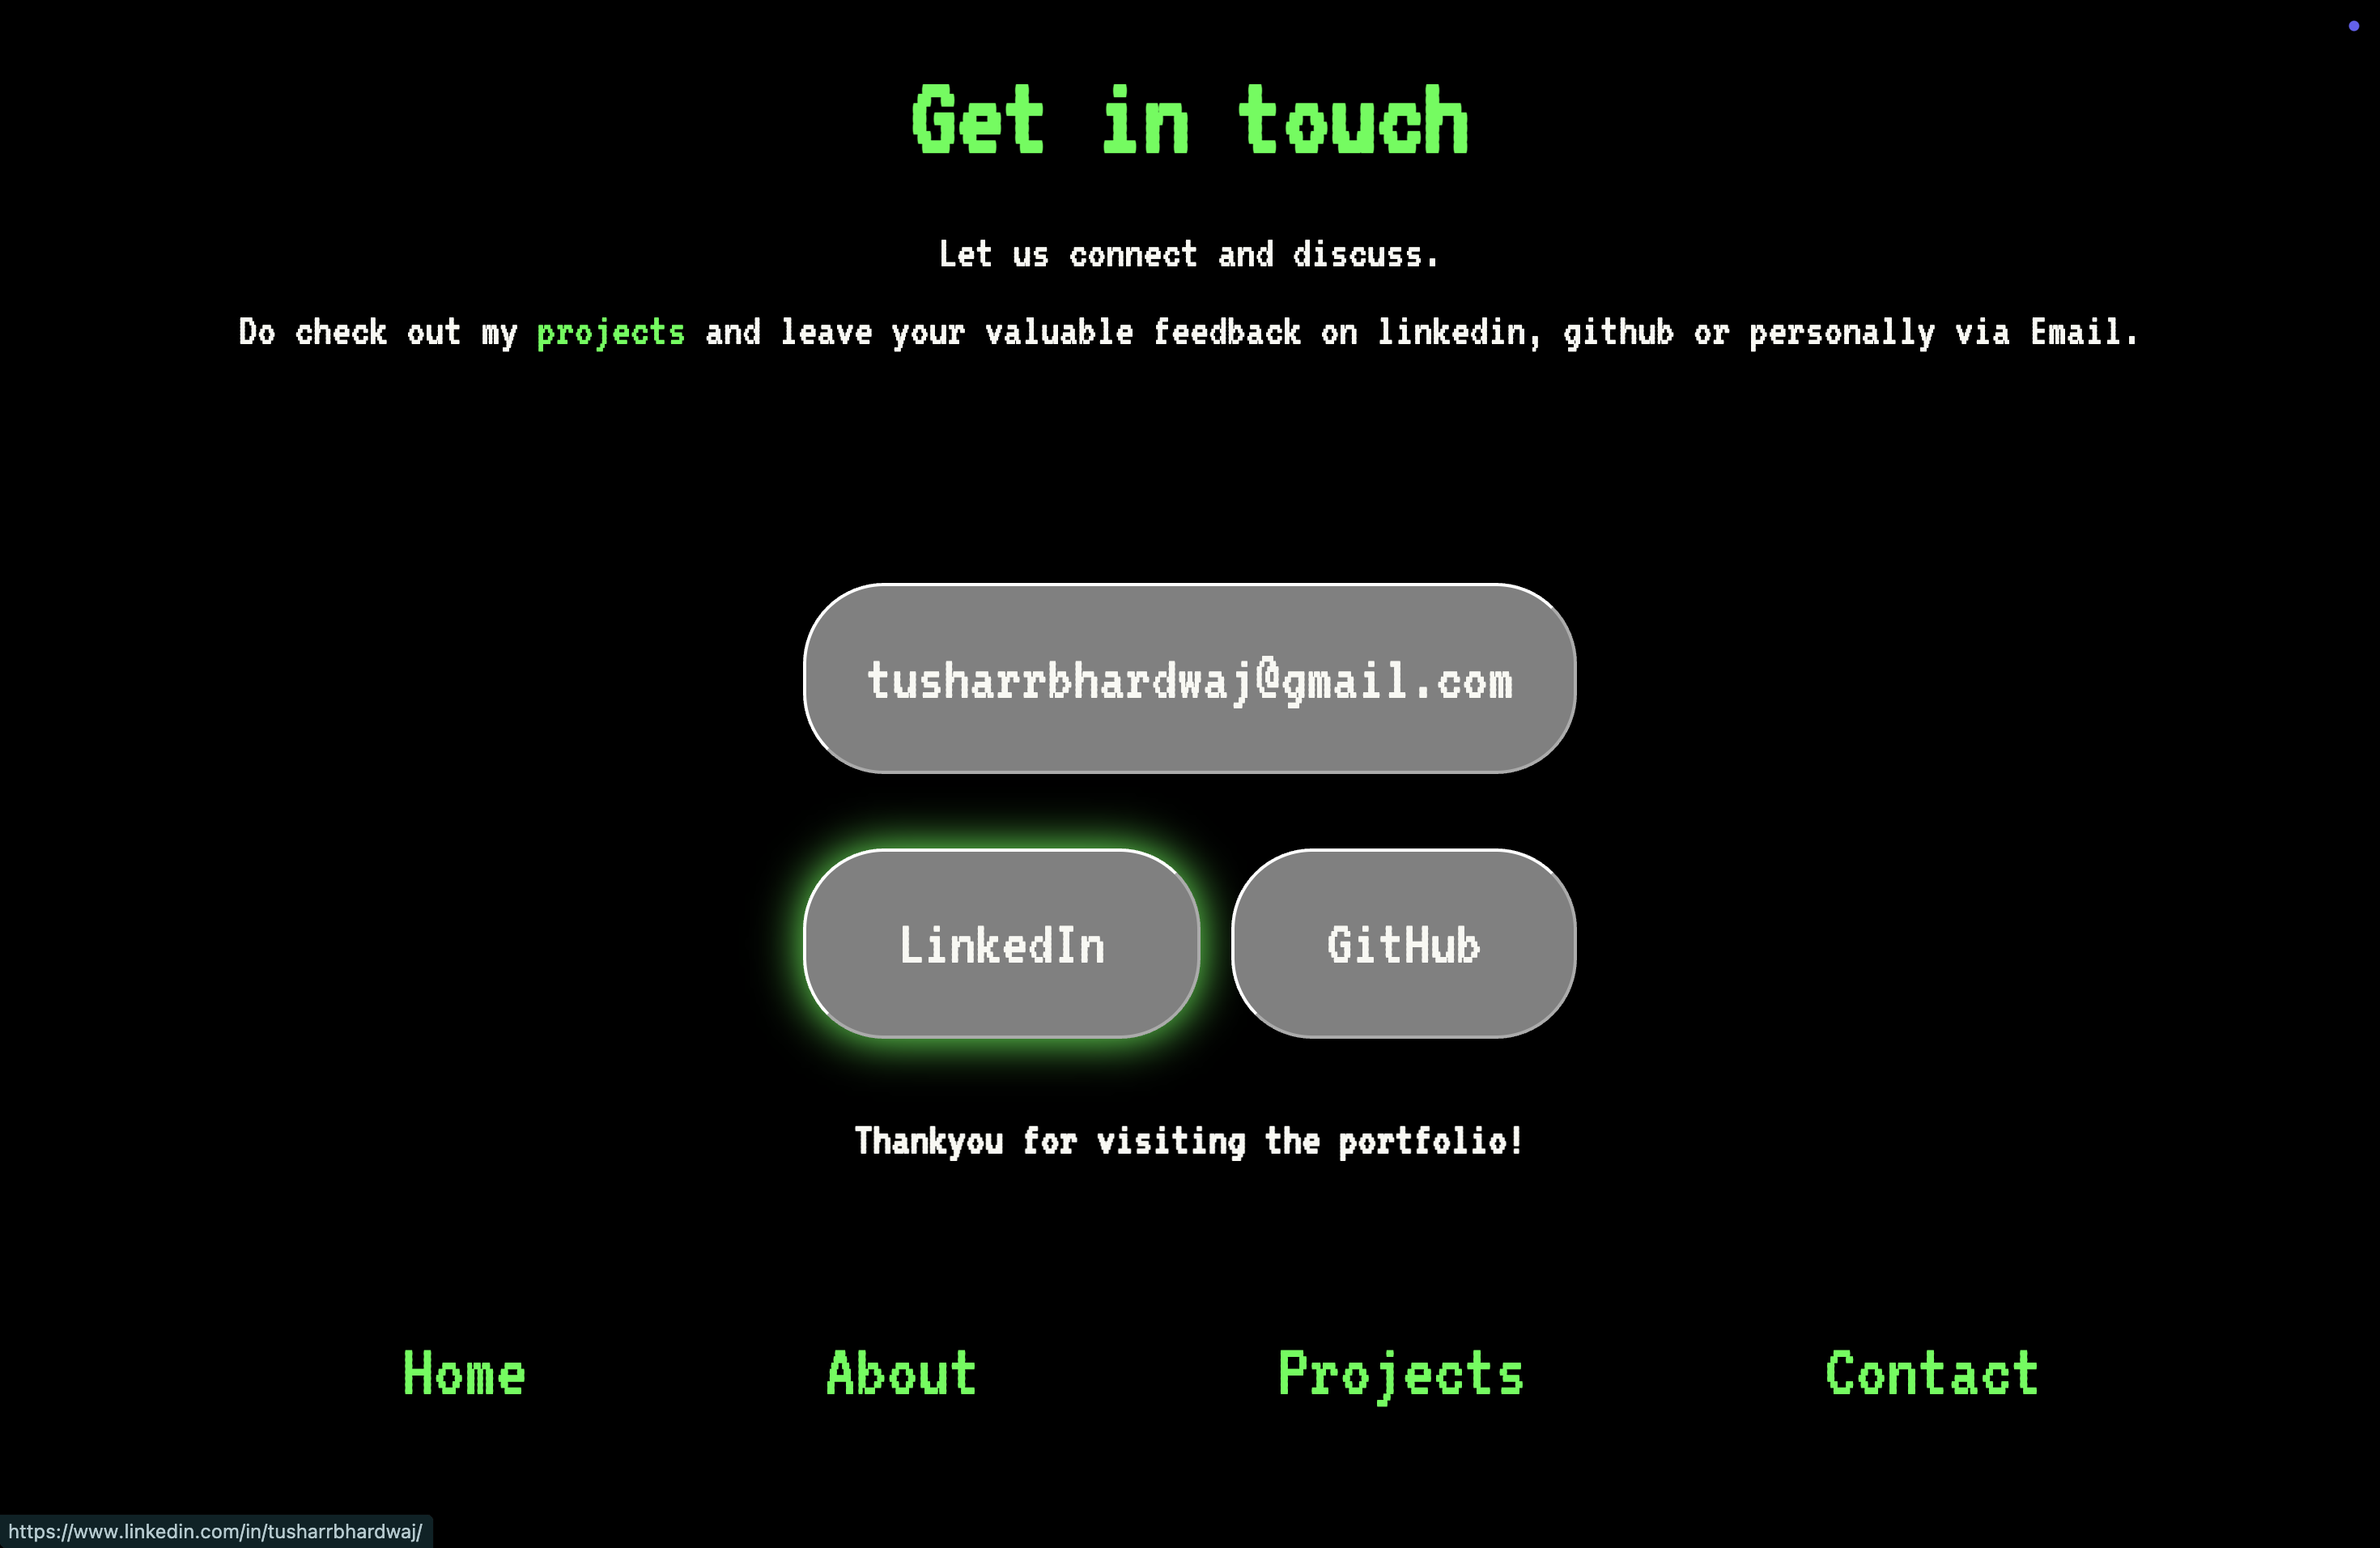
\includegraphics[width=1\linewidth]{webshots/contact.png}
    \end{minipage}
    \begin{minipage}{0.49\textwidth}
        \centering
        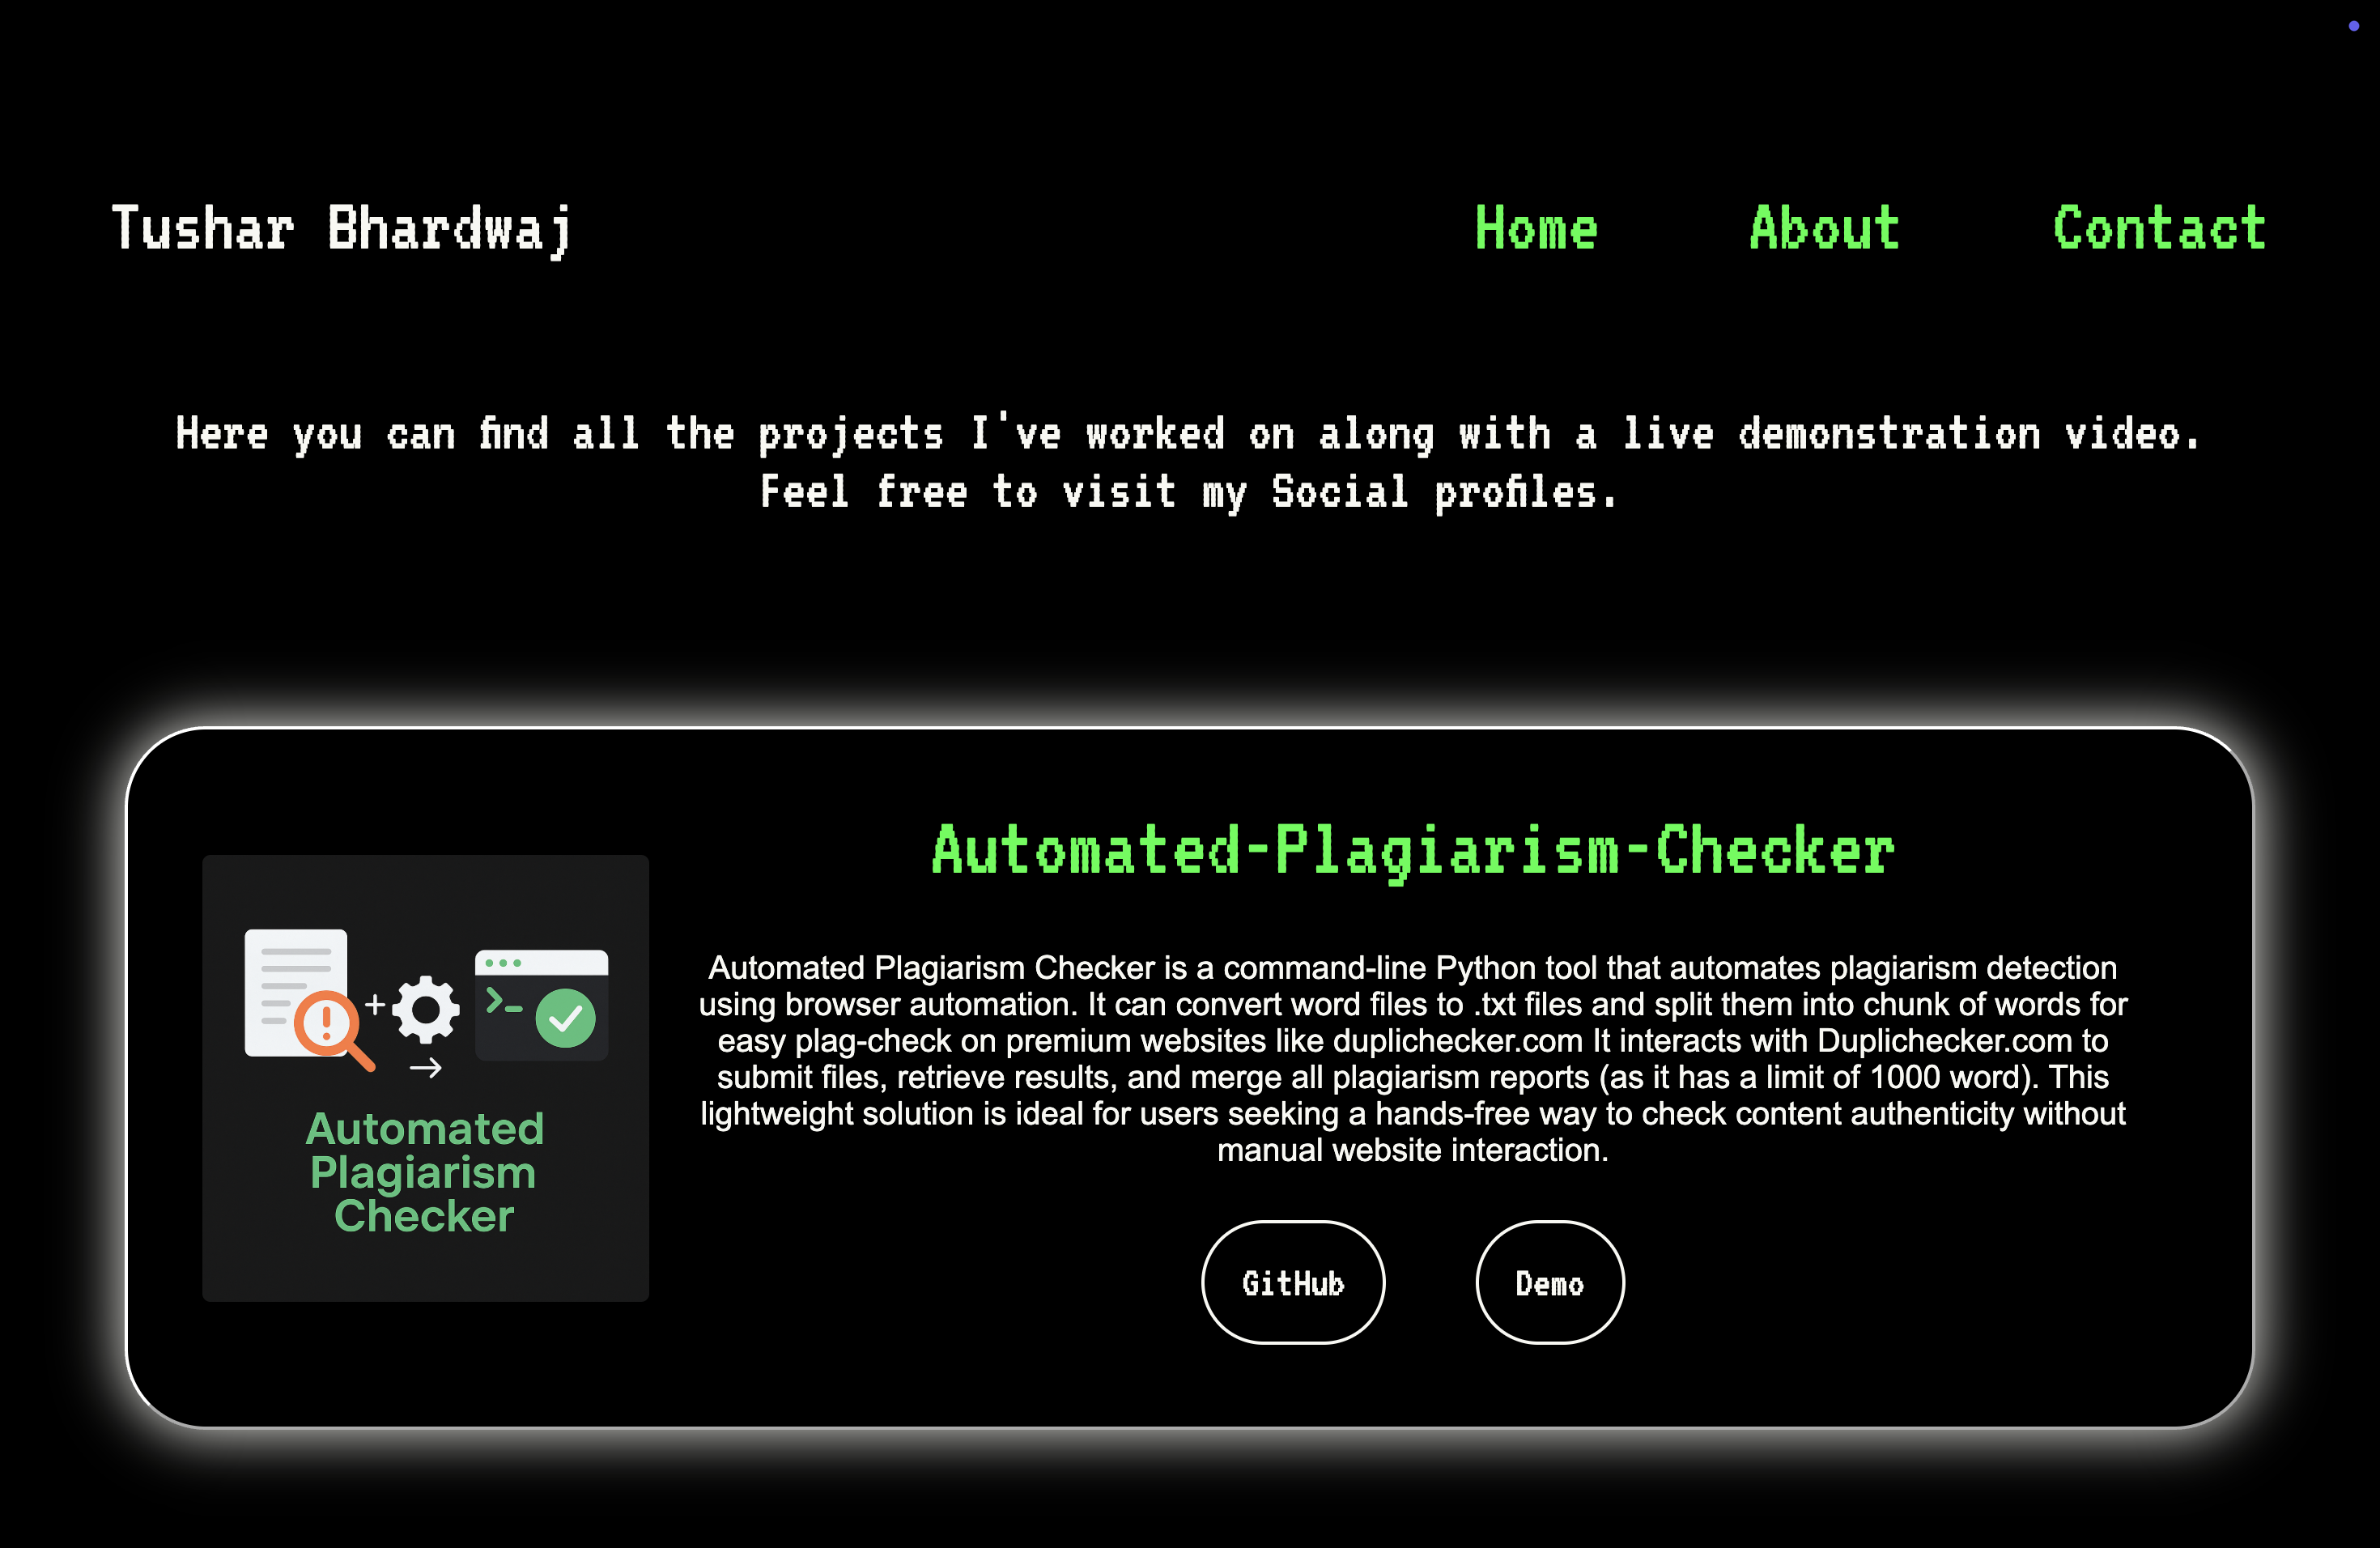
\includegraphics[width=1\linewidth]{webshots/projects.png}
    \end{minipage}
\end{figure}

\newpage
\section{Curriculum Vitae} \par

{\bf Link : \href{https://github.com/tusharrbhardwaj/CV/blob/main/Tushar_CV.pdf}{\color{blue}PDF}}\\
{\bf GitHub: \href{https://github.com/tusharrbhardwaj/CV}{\color{blue}Source Code}} \\ \par
This is my Curriculum Vitae, which is made in LaTeX using a template by Wilson Resume\cite{noauthor_latex_nodate} Further changes were made by editing the main file.\cite{alexander_baran-harper_latex_2014} This CV's .tex files are divided into two parts for a more organized presentation.\\
First file is the {\bf main.tex} file which consists of all the content that is displayed in the PDF. The other file is {\bf structure.tex} which contains all the packages and formatting of the document that can be seen in the PDF.\cite{noauthor_38_nodate} \\ \par
Following is the snapshot of the PDF for better understanding of the design and structure of the CV
\begin{figure}[h]
    \centering
    \begin{minipage}{0.49\textwidth}
        \centering
        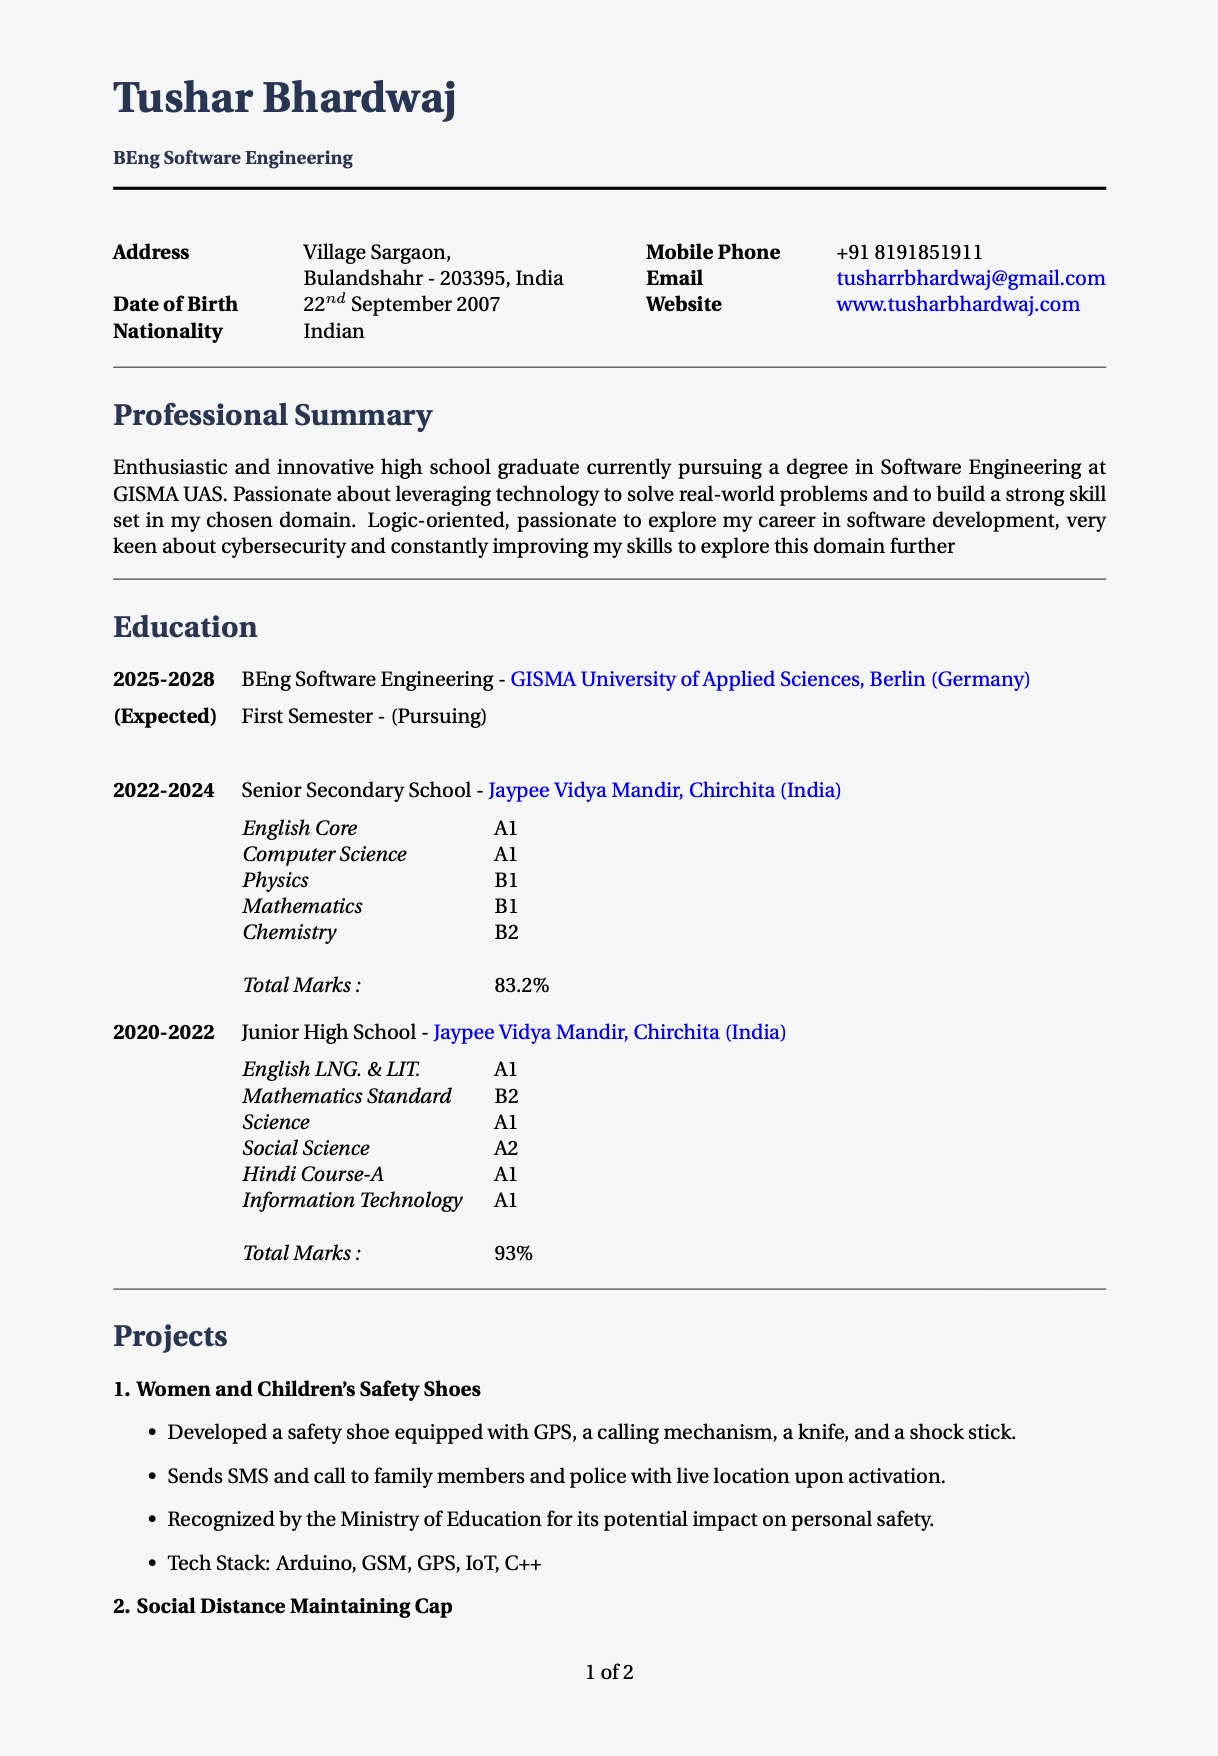
\includegraphics[width=1\linewidth]{CV/CV-pg1.jpeg}
    \end{minipage}
    \begin{minipage}{0.49\textwidth}
        \centering
        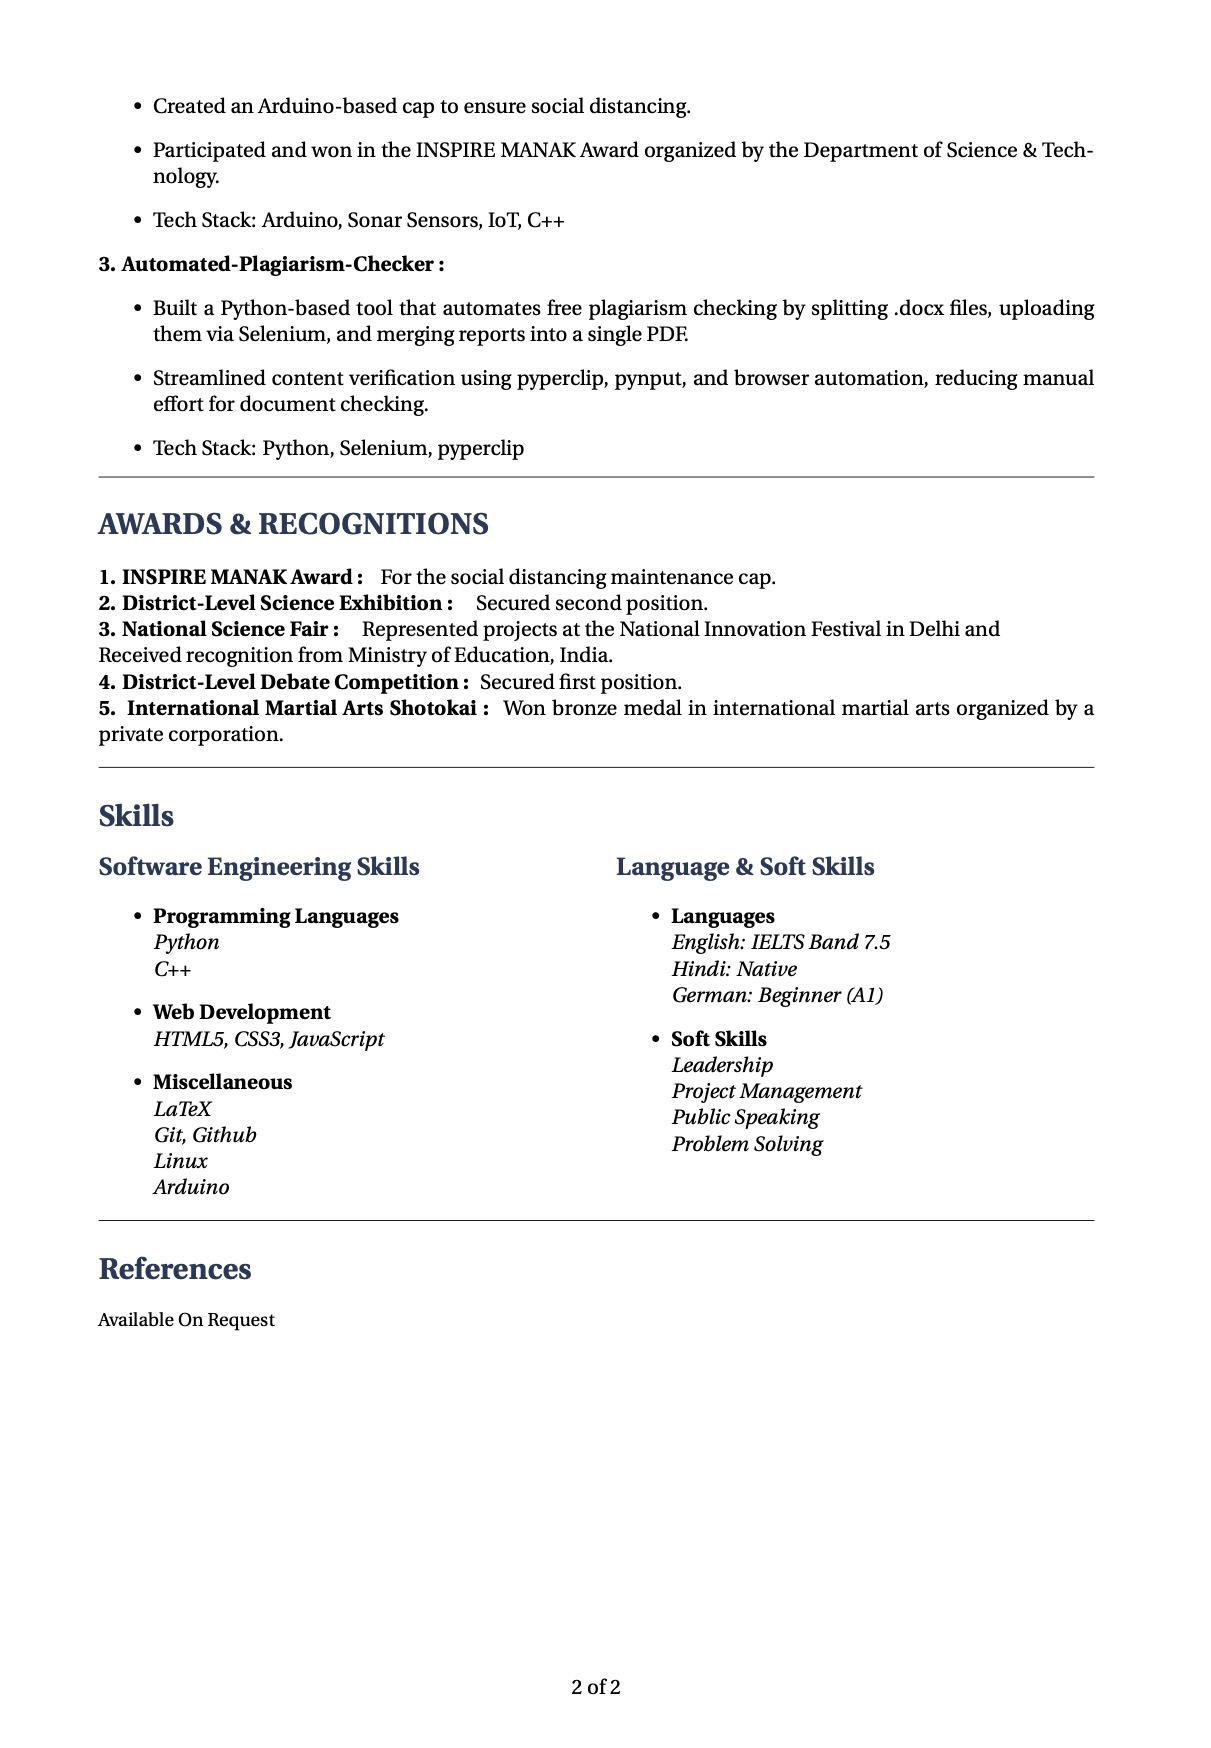
\includegraphics[width=1\linewidth]{CV/CV-pg2.jpeg}  
    \end{minipage}
\end{figure}

\newpage
\section{Automated Plagiarism Checker & Report Generator}
{\bf Link : \href{youtuve.com}{\color{blue}Demo Video}}\\
{\bf GitHub: \href{https://github.com/tusharrbhardwaj/Automated-Plagiarism-Checker}{\color{blue}Source Code}} \\ \par
Before diving deep into why and what this project is about, let's have some insight about the features of this tool. This is a full-fledged Python tool that:\\
\begin{itemize}
    \item Splits large '.docx files into \~n-word chunks 
    \item Automates browser interactions with Duplichecker using 'selenium'
    \item Uses 'pyperclip' + 'pynput' to simulate human-like copy-paste 
    \item Organizes chunked content and downloaded reports in folders 
    \item Merges all reports into one professional PDF using 'FPDF' 
    \item Saves time and reduces manual effort dramatically
\end{itemize}\\

Now the reason behind development of this project consists of more than problem which were solved one at a time.\\
The following table indicates towards the problem that arised and my solution towards them; which ultimately led to this automation tool.\\

\begin{tabular}{|m{6.5cm}|m{6.5cm}|}
    \hline
    {\bf Problems} & {\bf My solutions} \\ \hline
    Free tools limit text size  & Automatic file chunking \\ \hline
    Repetitive manual submission  & Smart naming + folder structure \\ \hline
    Hard to track which part was checked & Selenium-based automation \\ \hline
    Copy-paste errors & Clipboard simulation \\ \hline
    Unprofessional output & Merged, polished PDF report\\ \hline

\end{tabular}\\

\par This wasn’t just a technical experiment — it solved a real productivity challenge for me. And I believe it can help many others — students, researchers, content creators, or educators — facing similar issues. The type of result generated by this tool can be further understood with the help of few snapshots of program and reports.
\begin{figure}[h]
    \centering
    \begin{minipage}{0.49\textwidth}
        \centering
        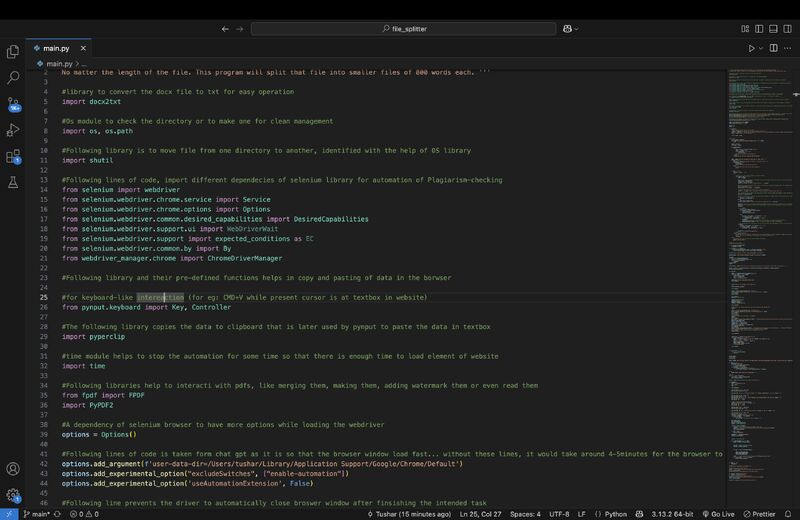
\includegraphics[width=1\linewidth]{Python project/code1.jpeg}
    \end{minipage}
    \begin{minipage}{0.49\textwidth}
        \centering
        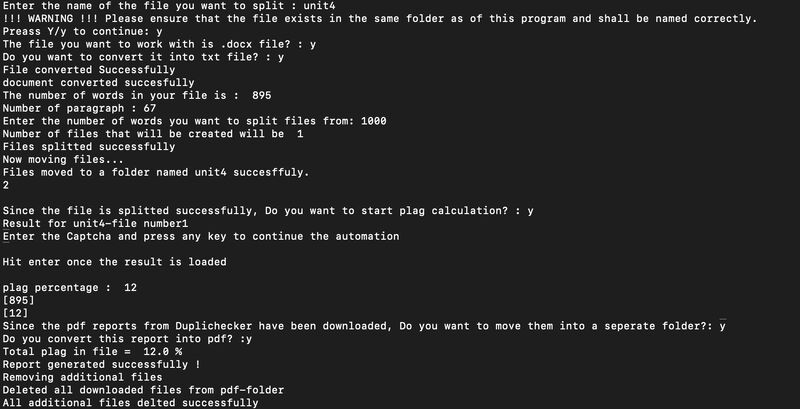
\includegraphics[width=1\linewidth]{Python project/code2.jpeg}  
    \end{minipage}
    %  \\
    % \begin{minipage}{0.49\textwidth}
    %     \centering
    %     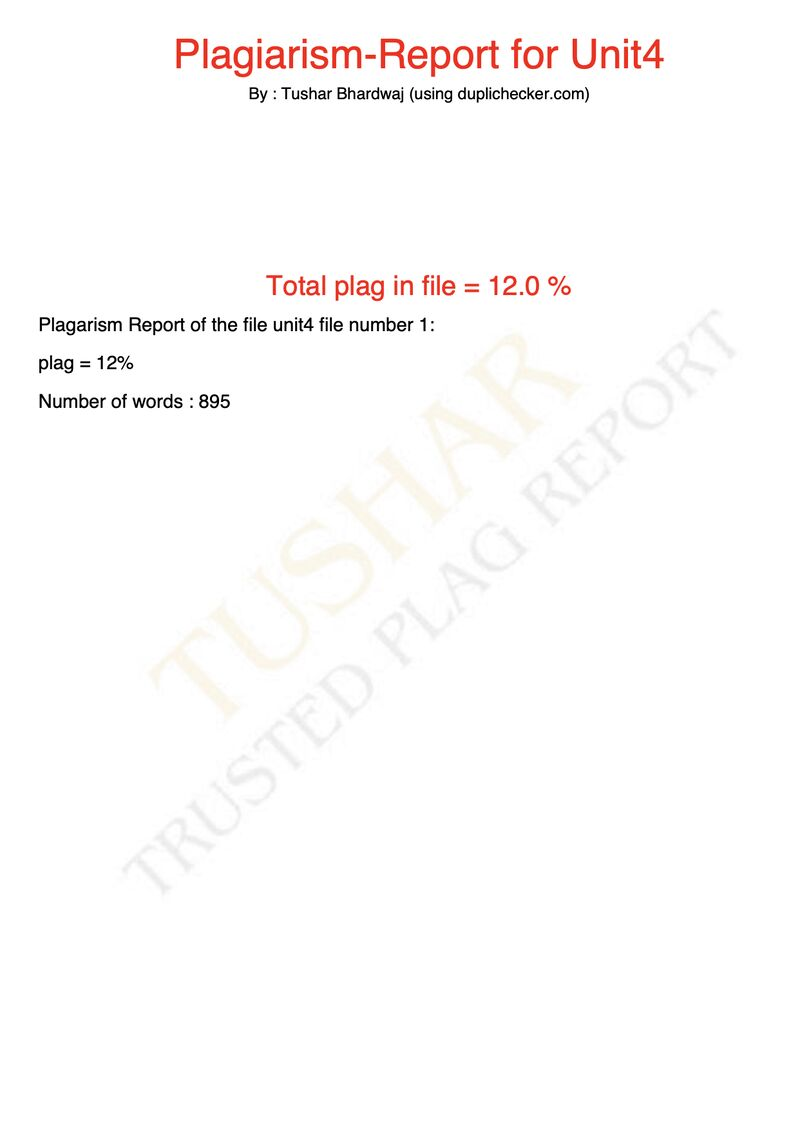
\includegraphics[width=0.75\linewidth]{Python project/report1.jpeg}
    % \end{minipage}
    % \begin{minipage}{0.49\textwidth}
    %     \centering
    %     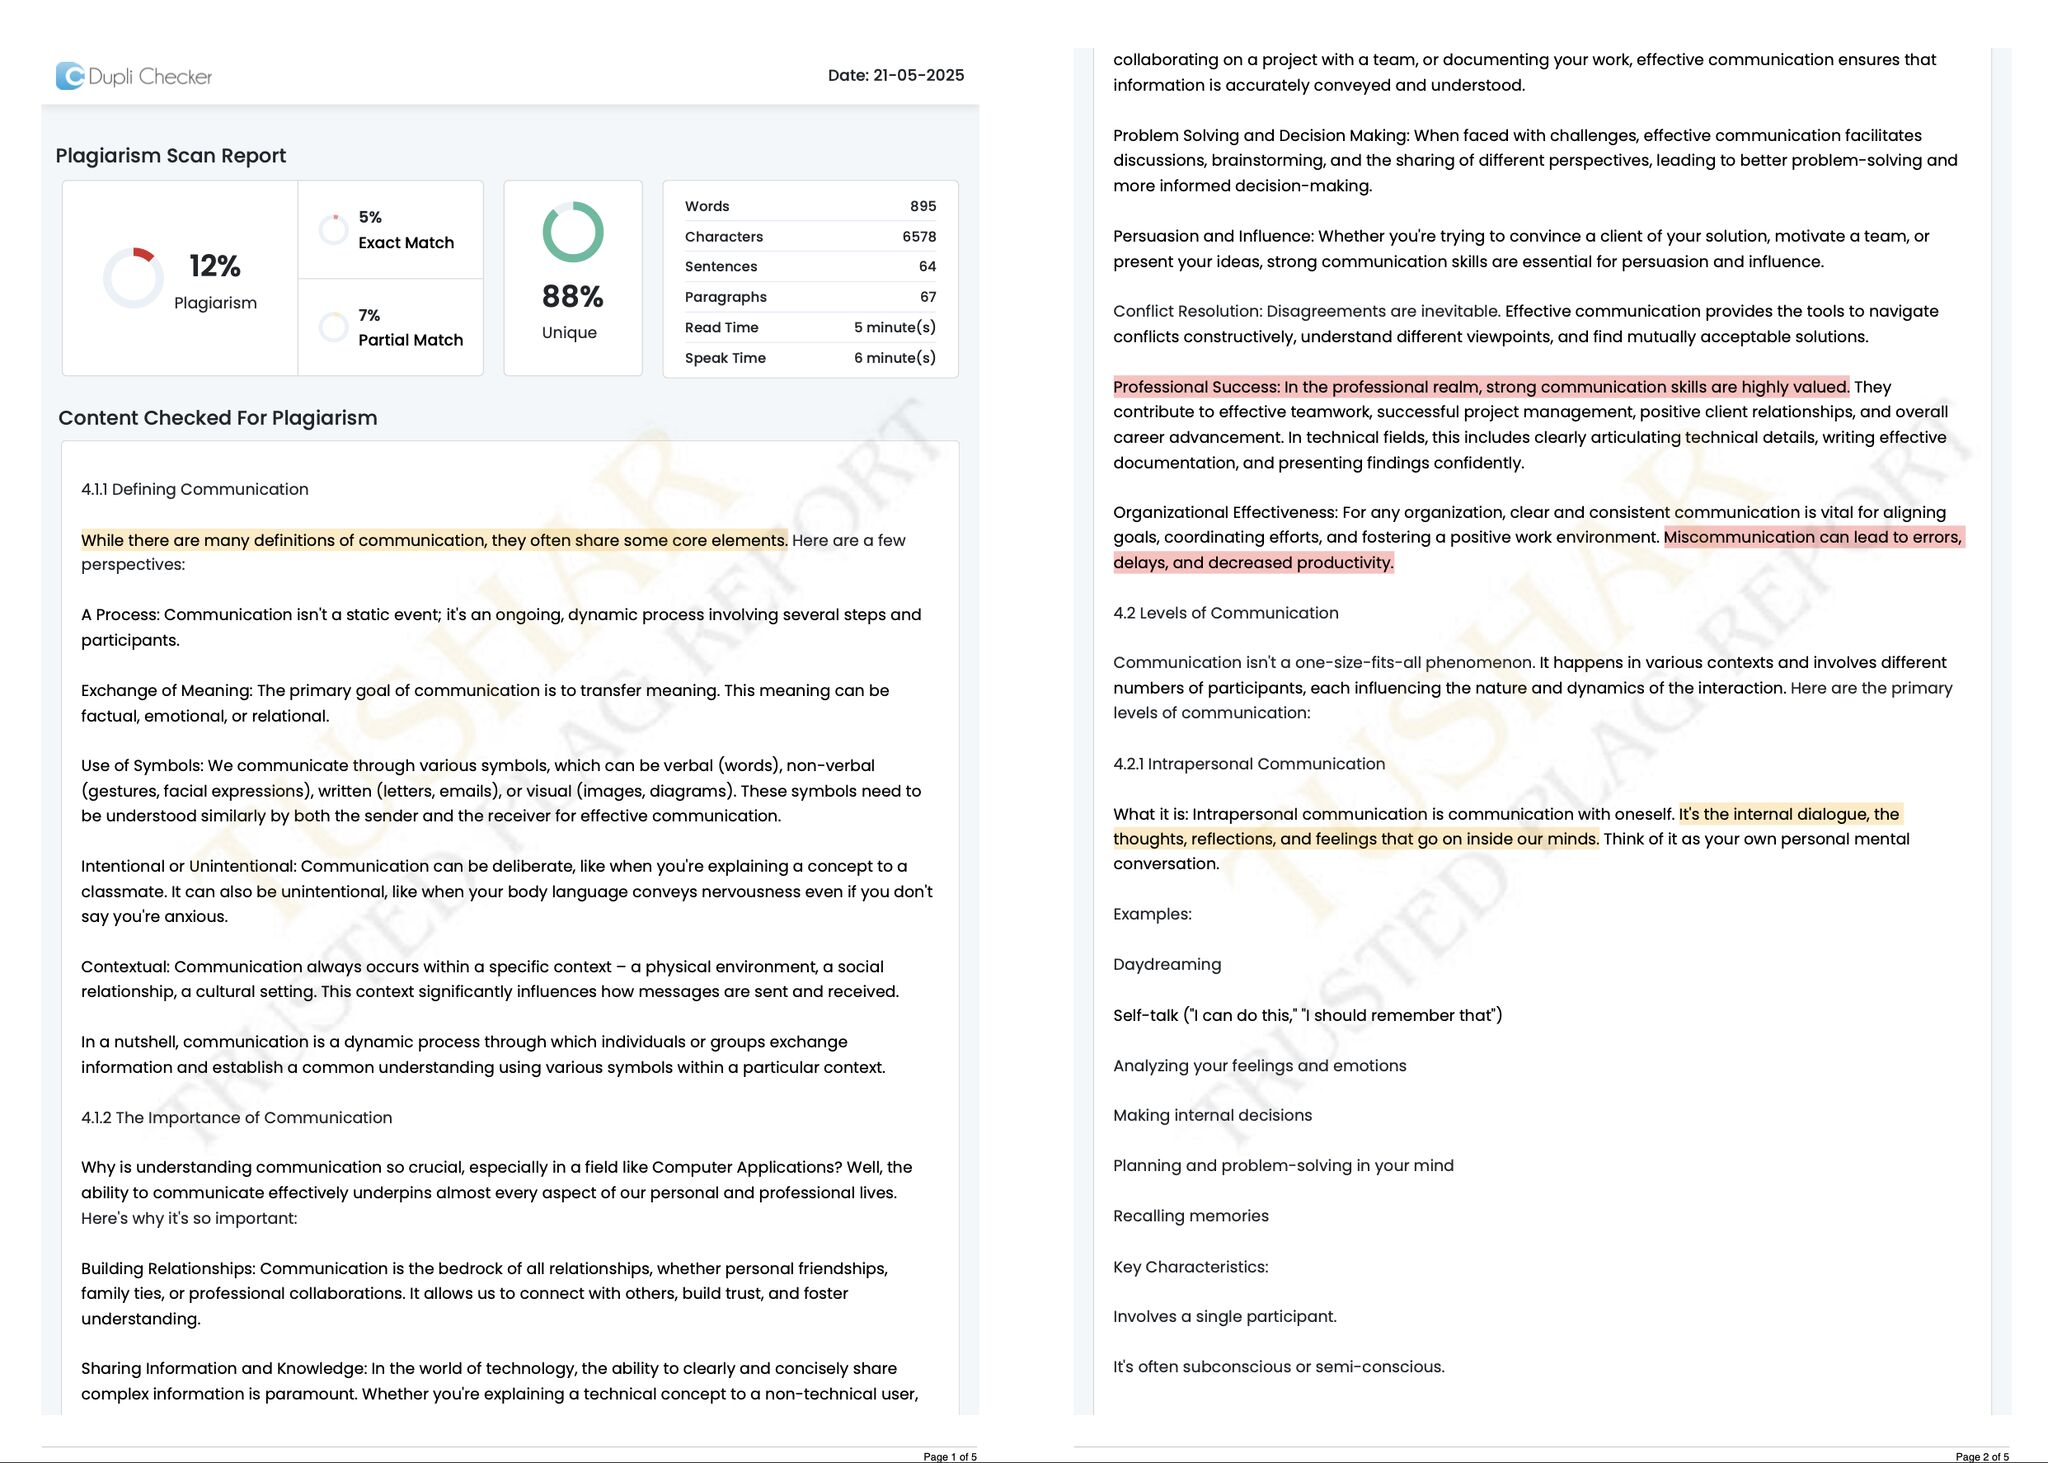
\includegraphics[width=1\linewidth]{Python project/report2.jpeg}
    % \end{minipage}
\end{figure}



\chapter{Portfolio Structure }
To keep the portfolio website simple, clean, and professional; I have divided the portfolio into three sections i.e., home page, about section, \& contact section and two pages i.e., index page and project page.\\
\par The Navigation consists of the hyperlinks to different section i.e. Projects, Contact and About. \\The navigation is the only part of the website which uses a small chunk of JavaScript to shrink into a menu-bar while on a device with small screen size.\\
This can be better seen in the following snapshots from the website. One is form the computer view and another is from a mobile phone.\\
\begin{figure}[h]
    \centering
    
\includegraphics[width=0.5\linewidth]{webshots/nav-comp.png}
    \caption*{Computer View of Navigation}\\
    \lab
    \vspace{0.75cm}
    \begin{minipage}{0.49\textwidth}
        \centering
        
\includegraphics[width=0.75\linewidth]{webshots/mob1.jpeg}
        \caption*{Mobile View Navigation (Collapsed)}
        \label*{}
    \end{minipage}
    \begin{minipage}{0.49\textwidth}
        \centering
        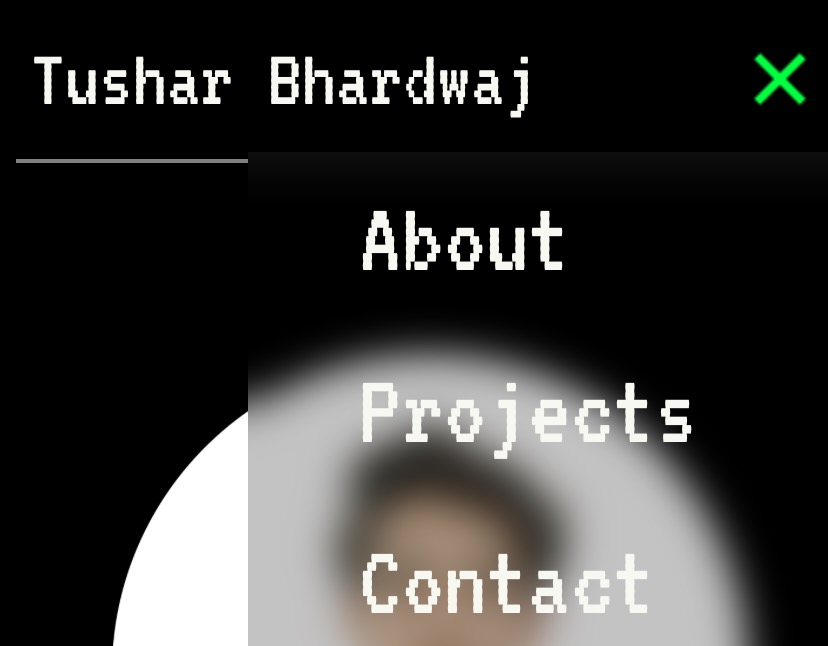
\includegraphics[width=0.75\linewidth]{webshots/mob2.jpeg}
        \caption*{Mobile View Navigation (Expanded)}
    \end{minipage}
\end{figure}\\

Moreover, the home page consists of a motto that better defines me.\\
The motto is \par {\bf "Just a dev, curious enough to turn ideas into code"}\\ with a clear and professional picture of me. This section of the website also has a CTA (Call to Action) button to download CV or reach my GitHub account directly.\par
The next section is about section which have a descriptive explanation on who I am and what my interests are. the about section is not very long but crisp enough to get a better insight of me.\\
Following the about section, there is a special section that only contains my ideology with CTA to contact. Here is the snapshot of the special section for thorough understanding of the design.\\
\begin{figure}[h]
    \vspace{0.5cm}
    \centering
    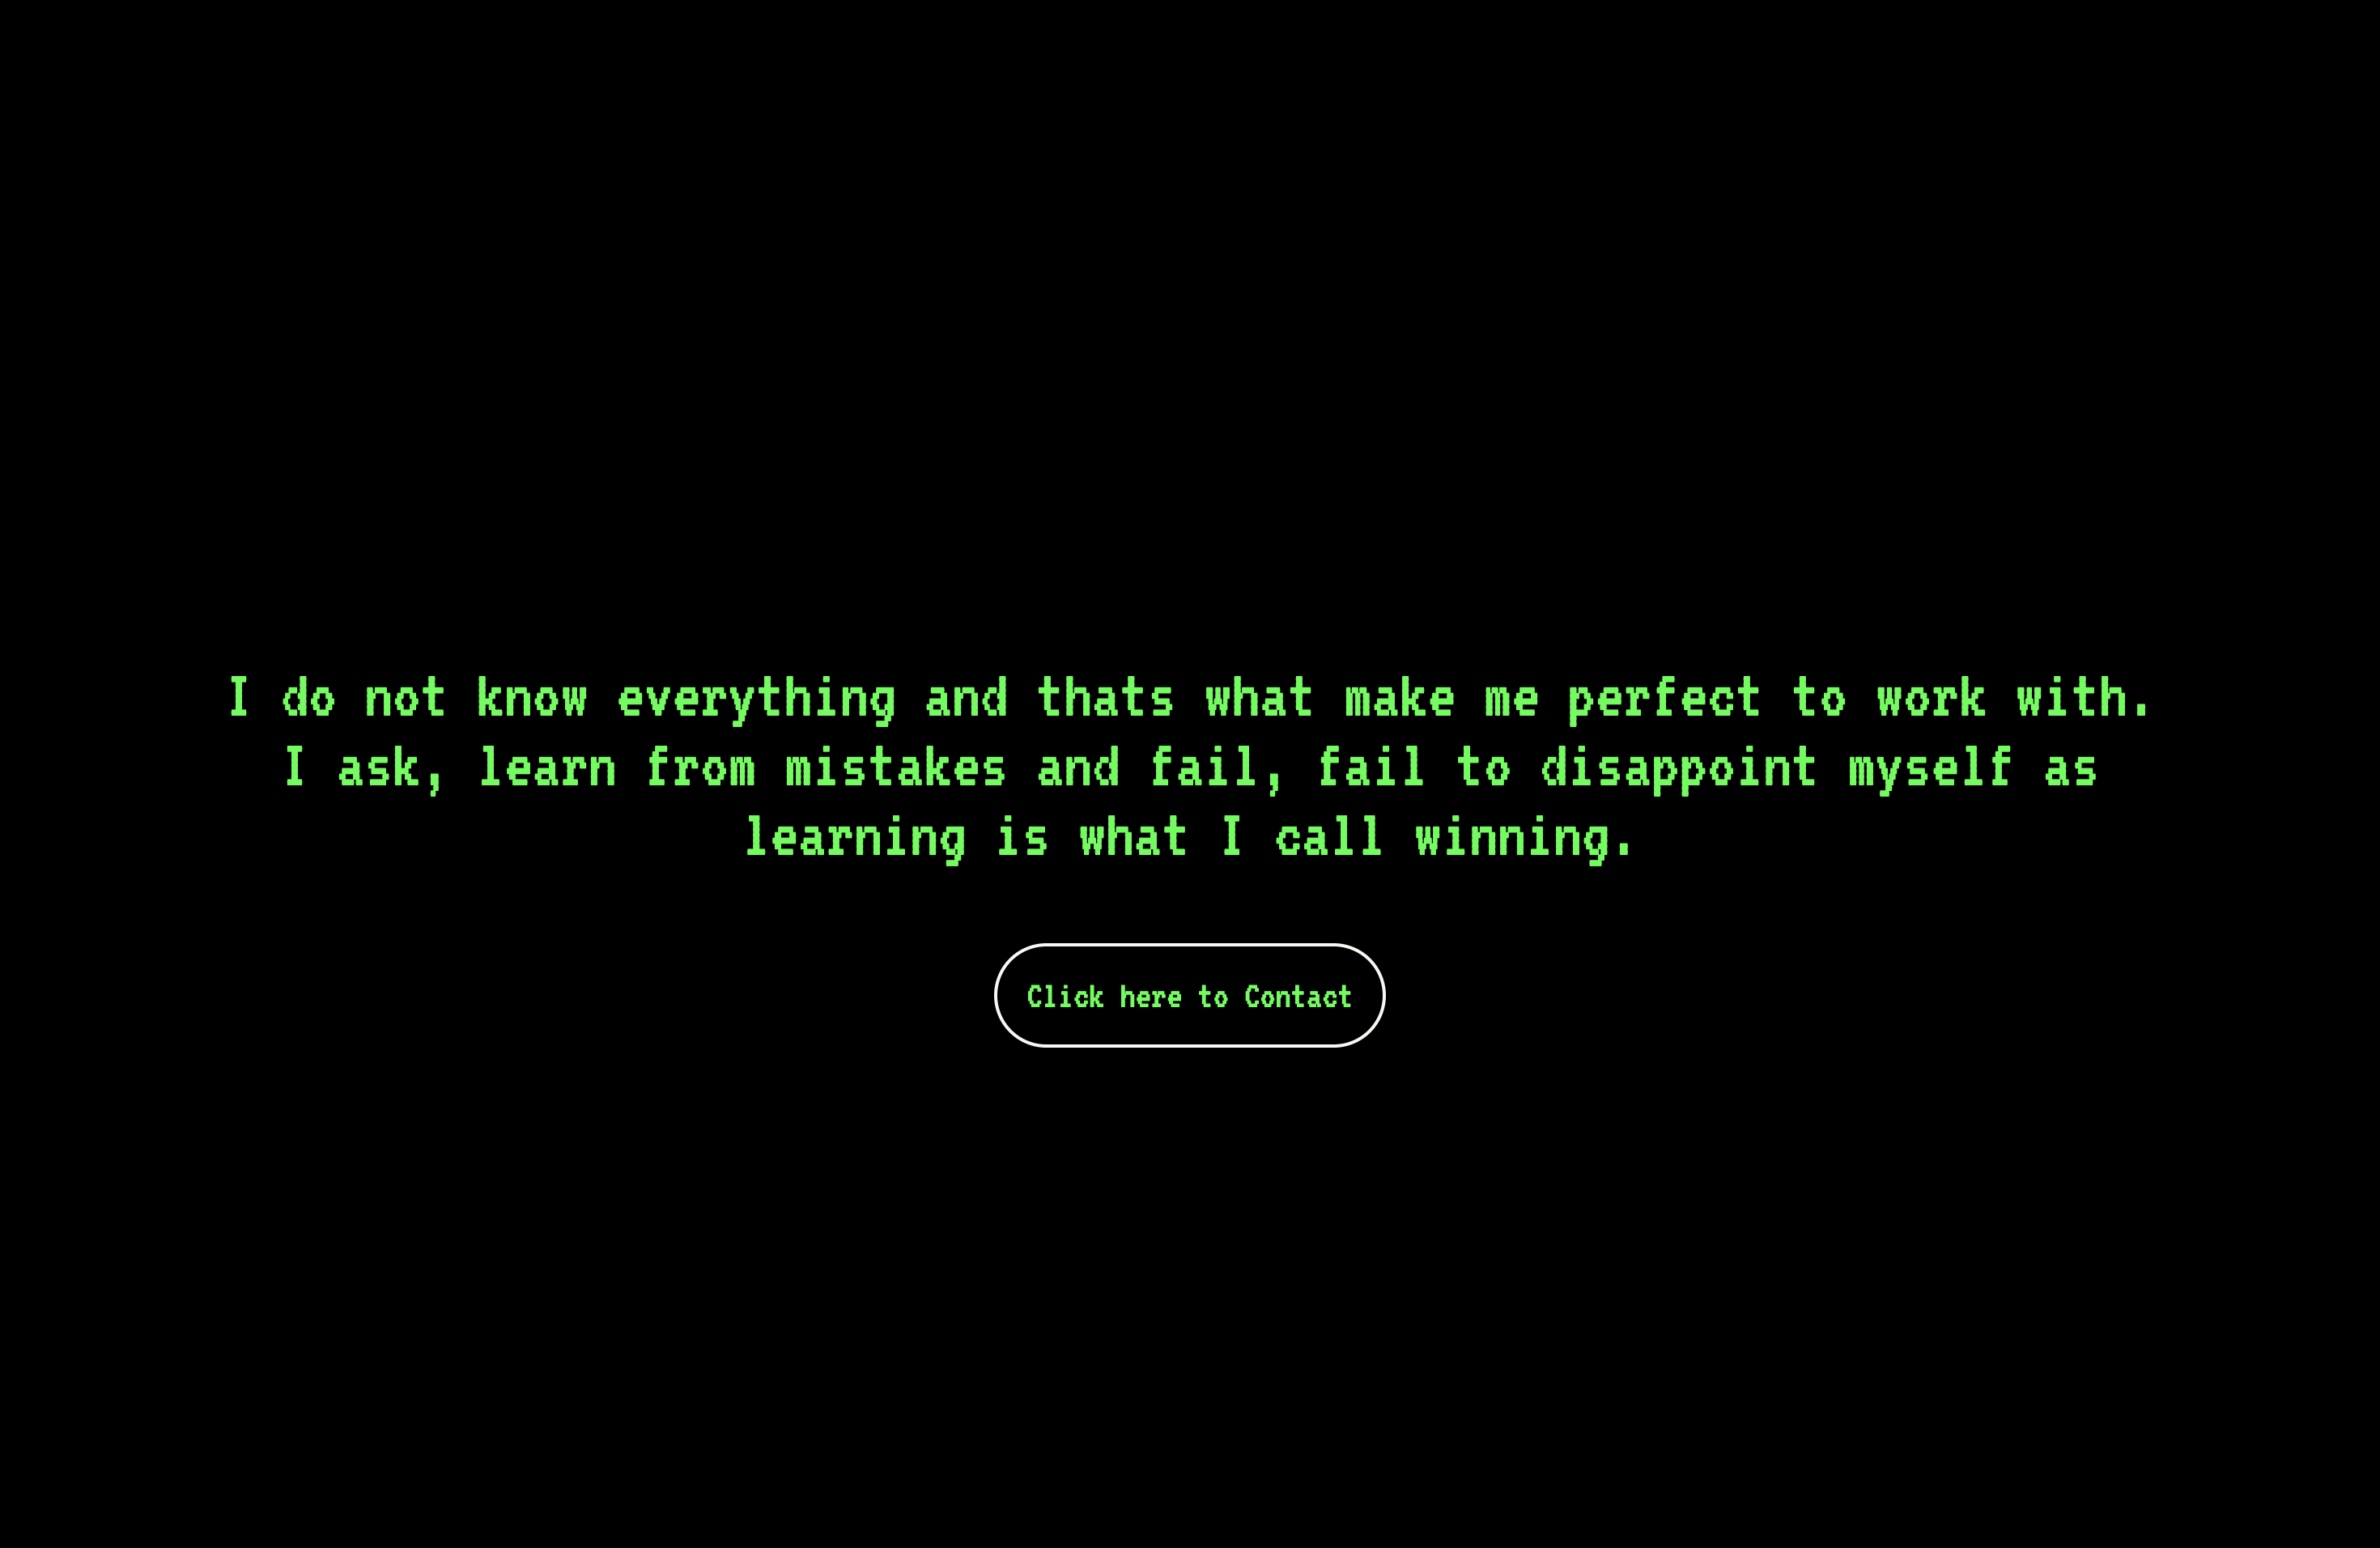
\includegraphics[width=0.75\linewidth]{webshots/special.png}
    \vspace{0.5cm}
\end{figure}
Then comes the contact section, which have the links to my socials like {\bf LinkedIn, GitHub, Email}, for ease of communication for feedback or collaborations.\par
Furthermore, the project page had been separated from the main page to make overall look visually appealing and clean while presenting almost all projects and bio-data I have about me. The projects are organized in a systematic manner allowing others to again insight on versatile tech-projects.\\
All the projects in the project page have their summary, a photo for visual representation, a demo button which leads to my YouTube channel having all the demo videos of my projects and a GitHub button which directs them to the source code of the particular project in GitHub.\\ This was the full the structure of my portfolio website.



\section{Design Choices}
To keep the website very simplistic and minimal, I chose the color theme to be of black color, however, at the same time I wanted the website to look tech-savvy and hence I chose a Greenish shade that is used in terminal and may feel smooth while looking at a computer screen. \\
Furthermore, To initialize the terminal feel to make it look more tech-savvy, I used terminal-like font from google fonts. However, for clear visibility of different attributes of this website I combined that font with normal sans-sarif font.\\
\par
The buttons on the website has a hover effect which looks like the background is glowing while hovering over the button. This was achieved through box shadows and it brought a show-room alike feel to different attributes to lure the viewer into clicking it or at least hovering over it.
\\ The other aspects of the design choices were discussed in portfolio-structure section.\par
Similar effects were brought in project section to maintain the consistency of the design which will ultimately enhance the user experience. 
% This section is bibliography section

\chapter{Tools \& Technology}
The website was made using {\bf HTML5, CSS3, and a chunk of JavaScript}. The IDE used to write the code of the website is Visual Studio Code using "liver server" extension to test the real-time working of the website.\\ Along with that a hosting service named {\bf netlify.com} was used to host the website on my personal domain i.e. {\bf tusharbhardwaj.com} which I rented from a domain provided {\bf name.com}.\\ \par
All the images used in the project section are AI generated along with few of the original image of the project that I clicked.\\ The profile picture is made using canvas and edited using a online website called {\bg bgremove.org}. \\ \par

To make the LaTeX CV and this report, an online text editor {\bf overleaf.com} has been used for clear and concise development of the module's assignment.\\
Furthermore, GitHub has been used for version-control and as the repository host for easy access to anyone visiting my online portfolio.

\chapter{Future Improvements}
I have a vision to take this portfolio and make it so strong that my chances for working-student position increase exponentially in any company.\\
Currently the demo button of the projects redirects the user to my YouTube channel which is currently empty, in future I'll be recording videos of the projects along with a short journey video to enhance the authenticity of the projects that I'm claiming as my own.\\ \par
Furthermore, I'm aiming to learn full stack development thoroughly and then apply my learning to my own portfolio. 


\chapter{Conclusion}
This project has been an enriching learning experience in not only constructing a technical portfolio but also learning the significance of personal presentation and branding in the world of technology. From this assignment, I created a professional portfolio webpage using web development software, produced a tidy and organized CV in LaTeX, and constructed a working automation project in Python.\\ \par

I also learned hands-on experience working with GitHub for version control and collaboration, as well as the value of documenting and presenting work. 
\\
Overall, this assignment has enhanced my professional and technical skills. I am more confident now in applying for working-student jobs and look forward to continuing to enhance my portfolio with new projects, features, and designs. \\ \par

\section{Links To This Report}
Link to this report's file source code and raw .tex file can be found on GitHub repository linked below. \\
{\bf Link : \href{https://github.com/tusharrbhardwaj/CS-Lab-Report}{\color{blue}Github}}\\


\bibliographystyle{plain}
\bibliography{refrencescslab}

\end{document}
